
\chapter{The Verilog and AST Frontends}
\label{chapter:verilog}

This chapter provides an overview of the implementation of the Yosys Verilog
and AST frontends. The Verilog frontend reads Verilog-2005 code and creates
an abstract syntax tree (AST) representation of the input. This AST representation
is then passed to the AST frontend that converts it to RTLIL data, as illustrated
in Fig.~\ref{fig:Verilog_flow}.

\begin{figure}[b!]
	\hfil
	\begin{tikzpicture}
		\tikzstyle{process} = [draw, fill=green!10, rectangle, minimum height=3em, minimum width=10em, node distance=5em, font={\ttfamily}]
		\tikzstyle{data} = [draw, fill=blue!10, ellipse, minimum height=3em, minimum width=7em, node distance=5em, font={\ttfamily}]

		\node[data]    (n1)               {Verilog Source};
		\node[process] (n2) [below of=n1] {Verilog Frontend};
		\node[data]    (n3) [below of=n2] {AST};
		\node[process] (n4) [below of=n3] {AST Frontend};
		\node[data]    (n5) [below of=n4] {RTLIL};

		\draw[-latex] (n1) -- (n2);
		\draw[-latex] (n2) -- (n3);
		\draw[-latex] (n3) -- (n4);
		\draw[-latex] (n4) -- (n5);

		\tikzstyle{details} = [draw, fill=yellow!5, rectangle, node distance=6cm, font={\ttfamily}]

		\node[details] (d1) [right of=n2] {\begin{minipage}{5cm}
			\hfil
			\begin{tikzpicture}
				\tikzstyle{subproc} = [draw, fill=green!10, rectangle, minimum height=2em, minimum width=10em, node distance=3em, font={\ttfamily}]
				\node (s0) {};
				\node[subproc] (s1) [below of=s0] {Preprocessor};
				\node[subproc] (s2) [below of=s1] {Lexer};
				\node[subproc] (s3) [below of=s2] {Parser};
				\node[node distance=3em] (s4) [below of=s3] {};
				\draw[-latex] (s0) -- (s1);
				\draw[-latex] (s1) -- (s2);
				\draw[-latex] (s2) -- (s3);
				\draw[-latex] (s3) -- (s4);
			\end{tikzpicture}
		\end{minipage}};

		\draw[dashed] (n2.north east) -- (d1.north west);
		\draw[dashed] (n2.south east) -- (d1.south west);

		\node[details] (d2) [right of=n4] {\begin{minipage}{5cm}
			\hfil
			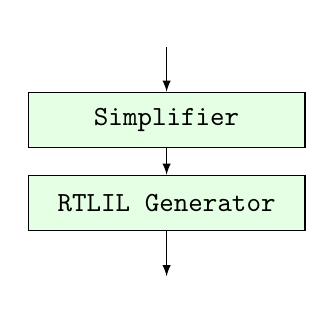
\begin{tikzpicture}
				\tikzstyle{subproc} = [draw, fill=green!10, rectangle, minimum height=2em, minimum width=10em, node distance=3em, font={\ttfamily}]
				\node (s0) {};
				\node[subproc] (s1) [below of=s0] {Simplifier};
				\node[subproc] (s2) [below of=s1] {RTLIL Generator};
				\node[node distance=3em] (s3) [below of=s2] {};
				\draw[-latex] (s0) -- (s1);
				\draw[-latex] (s1) -- (s2);
				\draw[-latex] (s2) -- (s3);
			\end{tikzpicture}
		\end{minipage}};

		\draw[dashed] (n4.north east) -- (d2.north west);
		\draw[dashed] (n4.south east) -- (d2.south west);

	\end{tikzpicture}
	\caption{Simplified Verilog to RTLIL data flow}
	\label{fig:Verilog_flow}
\end{figure}


\section{Transforming Verilog to AST}

The {\it Verilog frontend} converts the Verilog sources to an internal AST representation that closely resembles
the structure of the original Verilog code. The Verilog frontend consists of three components, the
{\it Preprocessor}, the {\it Lexer} and the {\it Parser}.

The source code to the Verilog frontend can be found in {\tt frontends/verilog/} in the Yosys source tree.

\subsection{The Verilog Preprocessor}

The Verilog preprocessor scans over the Verilog source code and interprets some of the Verilog compiler
directives such as \lstinline[language=Verilog]{`include}, \lstinline[language=Verilog]{`define} and
\lstinline[language=Verilog]{`ifdef}.

It is implemented as a C++ function that is passed a file descriptor as input and returns the
pre-processed Verilog code as a \lstinline[language=C++]{std::string}.

The source code to the Verilog Preprocessor can be found in {\tt
frontends/verilog/preproc.cc} in the Yosys source tree.

\subsection{The Verilog Lexer}

\begin{sloppypar}
The Verilog Lexer is written using the lexer generator {\it flex} \citeweblink{flex}. Its source code
can be found in {\tt frontends/verilog/verilog\_lexer.l} in the Yosys source tree.
The lexer does little more than identifying all keywords and literals
recognised by the Yosys Verilog frontend.
\end{sloppypar}

The lexer keeps track of the current location in the Verilog source code using
some global variables. These variables are used by the constructor of AST nodes
to annotate each node with the source code location it originated from.

\begin{sloppypar}
Finally the lexer identifies and handles special comments such as
``\lstinline[language=Verilog]{// synopsys translate_off}'' and
``\lstinline[language=Verilog]{// synopsys full_case}''. (It is recommended to
use \lstinline[language=Verilog]{`ifdef} constructs instead of the Synsopsys
translate\_on/off comments and attributes such as
\lstinline[language=Verilog]{(* full_case *)} over ``\lstinline[language=Verilog]{// synopsys full_case}''
whenever possible.)
\end{sloppypar}

\subsection{The Verilog Parser}

The Verilog Parser is written using the parser generator {\it bison} \citeweblink{bison}. Its source code
can be found in {\tt frontends/verilog/verilog\_parser.y} in the Yosys source tree.

It generates an AST using the \lstinline[language=C++]{AST::AstNode} data structure
defined in {\tt frontends/ast/ast.h}. An \lstinline[language=C++]{AST::AstNode} object has
the following properties:

%%%%%%%%%%%%%%%%%%%%%%%%%%%%%%%%%%%%%%%%%%%%%%%%%%%%%%%%%%%%%%%%%%

\begin{table}[b!]
\hfil
\begin{tabular}{>{\raggedright\arraybackslash}p{7cm}>{\raggedright\arraybackslash}p{8cm}}
AST Node Type & Corresponding Verilog Construct \\
\hline
\hline
\arrayrulecolor{gray}
{\tt AST\_NONE} & This Node type should never be used. \\
\hline
%
{\tt AST\_DESIGN} & This node type is used for the top node of the AST tree. It
has no corresponding Verilog construct. \\
\hline
%
{\tt AST\_MODULE},
{\tt AST\_TASK},
{\tt AST\_FUNCTION} &
\lstinline[language=Verilog];module;,
\lstinline[language=Verilog];task; and
\lstinline[language=Verilog];function; \\
\hline
%
{\tt AST\_WIRE} &
\lstinline[language=Verilog];input;,
\lstinline[language=Verilog];output;,
\lstinline[language=Verilog];wire;,
\lstinline[language=Verilog];reg; and
\lstinline[language=Verilog];integer; \\
\hline
%
{\tt AST\_MEMORY}  &
Verilog Arrays \\
\hline
%
{\tt AST\_AUTOWIRE} &
Created by the simplifier when an undeclared signal name is used. \\
\hline
%
{\tt AST\_PARAMETER},
{\tt AST\_LOCALPARAM} &
\lstinline[language=Verilog];parameter; and
\lstinline[language=Verilog];localparam; \\
\hline
%
{\tt AST\_PARASET} &
Parameter set in cell instantiation \\
\hline
%
{\tt AST\_ARGUMENT} &
Port connection in cell instantiation \\
\hline
%
{\tt AST\_RANGE} &
Bit-Index in a signal or element index in array \\
\hline
%
{\tt AST\_CONSTANT} &
A literal value \\
\hline
%
{\tt AST\_CELLTYPE} &
The type of cell in cell instantiation \\
\hline
%
{\tt AST\_IDENTIFIER} &
An Identifier (signal name in expression or cell/task/etc. name in other contexts) \\
\hline
%
{\tt AST\_PREFIX} &
Construct an identifier in the form {\tt <prefix>[<index>].<suffix>} (used only in
advanced generate constructs) \\
\hline
%
{\tt AST\_FCALL},
{\tt AST\_TCALL} &
Call to function or task \\
\hline
%
{\tt AST\_TO\_SIGNED},
{\tt AST\_TO\_UNSIGNED} &
The \lstinline[language=Verilog];$signed(); and
\lstinline[language=Verilog];$unsigned(); functions \\
\hline
\end{tabular}
\caption{AST node types with their corresponding Verilog constructs. \\ (continued on next page)}
\label{tab:Verilog_AstNodeType}
\end{table}

\begin{table}[t!]
\ContinuedFloat
\hfil
\begin{tabular}{>{\raggedright\arraybackslash}p{7cm}>{\raggedright\arraybackslash}p{8cm}}
AST Node Type & Corresponding Verilog Construct \\
\hline
\hline
\arrayrulecolor{gray}
{\tt AST\_CONCAT}
{\tt AST\_REPLICATE} &
The \lstinline[language=Verilog];{...}; and
\lstinline[language=Verilog];{...{...}}; operators \\
\hline
%
{\tt AST\_BIT\_NOT},
{\tt AST\_BIT\_AND},
{\tt AST\_BIT\_OR},
{\tt AST\_BIT\_XOR},
{\tt AST\_BIT\_XNOR} &
The bitwise operators \break
\lstinline[language=Verilog];~;,
\lstinline[language=Verilog];&;,
\lstinline[language=Verilog];|;,
\lstinline[language=Verilog];^; and
\lstinline[language=Verilog];~^; \\
\hline
%
{\tt AST\_REDUCE\_AND},
{\tt AST\_REDUCE\_OR},
{\tt AST\_REDUCE\_XOR},
{\tt AST\_REDUCE\_XNOR} &
The unary reduction operators \break
\lstinline[language=Verilog];~;,
\lstinline[language=Verilog];&;,
\lstinline[language=Verilog];|;,
\lstinline[language=Verilog];^; and
\lstinline[language=Verilog];~^; \\
\hline
%
{\tt AST\_REDUCE\_BOOL} &
Conversion from multi-bit value to boolean value
(equivalent to {\tt AST\_REDUCE\_OR}) \\
\hline
%
{\tt AST\_SHIFT\_LEFT},
{\tt AST\_SHIFT\_RIGHT},
{\tt AST\_SHIFT\_SLEFT},
{\tt AST\_SHIFT\_SRIGHT} &
The shift operators \break
\lstinline[language=Verilog];<<;,
\lstinline[language=Verilog];>>;,
\lstinline[language=Verilog];<<<; and
\lstinline[language=Verilog];>>>; \\
\hline
%
{\tt AST\_LT},
{\tt AST\_LE},
{\tt AST\_EQ},
{\tt AST\_NE},
{\tt AST\_GE},
{\tt AST\_GT} &
The relational operators \break
\lstinline[language=Verilog];<;,
\lstinline[language=Verilog];<=;,
\lstinline[language=Verilog];==;,
\lstinline[language=Verilog];!=;,
\lstinline[language=Verilog];>=; and
\lstinline[language=Verilog];>; \\
\hline
%
{\tt AST\_ADD},
{\tt AST\_SUB},
{\tt AST\_MUL},
{\tt AST\_DIV},
{\tt AST\_MOD},
{\tt AST\_POW} &
The binary operators \break
\lstinline[language=Verilog];+;,
\lstinline[language=Verilog];-;,
\lstinline[language=Verilog];*;,
\lstinline[language=Verilog];/;,
\lstinline[language=Verilog];%; and
\lstinline[language=Verilog];**; \\
\hline
%
{\tt AST\_POS},
{\tt AST\_NEG} &
The prefix operators
\lstinline[language=Verilog];+; and
\lstinline[language=Verilog];-; \\
\hline
%
{\tt AST\_LOGIC\_AND},
{\tt AST\_LOGIC\_OR},
{\tt AST\_LOGIC\_NOT} &
The logic operators
\lstinline[language=Verilog];&&;,
\lstinline[language=Verilog];||; and
\lstinline[language=Verilog];!; \\
\hline
%
{\tt AST\_TERNARY} &
The ternary \lstinline[language=Verilog];?:;-operator \\
\hline
%
{\tt AST\_MEMRD}
{\tt AST\_MEMWR} &
Read and write memories. These nodes are generated by
the AST simplifier for writes/reads to/from Verilog arrays. \\
\hline
%
{\tt AST\_ASSIGN} &
An \lstinline[language=Verilog];assign; statement \\
\hline
%
{\tt AST\_CELL} &
A cell instantiation \\
\hline
%
{\tt AST\_PRIMITIVE} &
A primitive cell (\lstinline[language=Verilog];and;,
\lstinline[language=Verilog];nand;,
\lstinline[language=Verilog];or;, etc.) \\
\hline
%
{\tt AST\_ALWAYS},
{\tt AST\_INITIAL} &
Verilog \lstinline[language=Verilog];always;- and \lstinline[language=Verilog];initial;-blocks \\
\hline
%
{\tt AST\_BLOCK} &
A \lstinline[language=Verilog];begin;-\lstinline[language=Verilog];end;-block \\
\hline
%
{\tt AST\_ASSIGN\_EQ}.
{\tt AST\_ASSIGN\_LE} &
Blocking (\lstinline[language=Verilog];=;) and nonblocking (\lstinline[language=Verilog];<=;)
assignments within an \lstinline[language=Verilog];always;- or \lstinline[language=Verilog];initial;-block \\
\hline
%
{\tt AST\_CASE}.
{\tt AST\_COND},
{\tt AST\_DEFAULT} &
The \lstinline[language=Verilog];case; (\lstinline[language=Verilog];if;) statements, conditions within a case
and the default case respectively \\
\hline
%
{\tt AST\_FOR} &
A \lstinline[language=Verilog];for;-loop with an
\lstinline[language=Verilog];always;- or
\lstinline[language=Verilog];initial;-block \\
\hline
%
{\tt AST\_GENVAR},
{\tt AST\_GENBLOCK},
{\tt AST\_GENFOR},
{\tt AST\_GENIF} &
The \lstinline[language=Verilog];genvar; and
\lstinline[language=Verilog];generate; keywords and
\lstinline[language=Verilog];for; and \lstinline[language=Verilog];if; within a
generate block. \\
\hline
%
{\tt AST\_POSEDGE},
{\tt AST\_NEGEDGE},
{\tt AST\_EDGE} &
Event conditions for \lstinline[language=Verilog];always; blocks. \\
\hline
\end{tabular}
\caption{AST node types with their corresponding Verilog constructs. \\ (continuation from previous page)}
\label{tab:Verilog_AstNodeTypeCont}
\end{table}

%%%%%%%%%%%%%%%%%%%%%%%%%%%%%%%%%%%%%%%%%%%%%%%%%%%%%%%%%%%%%%%%%%

\begin{itemize}
\item {\bf The node type} \\
This enum (\lstinline[language=C++]{AST::AstNodeType}) specifies the role of the node.
Table~\ref{tab:Verilog_AstNodeType} contains a list of all node types.
\item {\bf The child nodes} \\
This is a list of pointers to all children in the abstract syntax tree.
\item {\bf Attributes} \\
As almost every AST node might have Verilog attributes assigned to it, the
\lstinline[language=C++]{AST::AstNode} has direct support for attributes. Note that the
attribute values are again AST nodes.
\item {\bf Node content} \\
Each node might have additional content data. A series of member variables exist to hold such data.
For example the member \lstinline[language=C++]{std::string str} can hold a string value and is
used e.g.~in the {\tt AST\_IDENTIFIER} node type to store the identifier name.
\item {\bf Source code location} \\
Each \lstinline[language=C++]{AST::AstNode} is automatically annotated with the current
source code location by the \lstinline[language=C++]{AST::AstNode} constructor. It is
stored in the \lstinline[language=C++]{std::string filename} and \lstinline[language=C++]{int linenum}
member variables.
\end{itemize}

The \lstinline[language=C++]{AST::AstNode} constructor can be called with up to
two child nodes that are automatically added to the list of child nodes for the new object.
This simplifies the creation of AST nodes for simple expressions a bit. For example the bison
code for parsing multiplications:

\begin{lstlisting}[numbers=left,frame=single]
        basic_expr '*' attr basic_expr {
                $$ = new AstNode(AST_MUL, $1, $4);
                append_attr($$, $3);
        } |
\end{lstlisting}

The generated AST data structure is then passed directly to the AST frontend
that performs the actual conversion to RTLIL.

Note that the Yosys command {\tt read\_verilog} provides the options {\tt -yydebug}
and {\tt -dump\_ast} that can be used to print the parse tree or abstract syntax tree
respectively.

\section{Transforming AST to RTLIL}

The {\it AST Frontend} converts a set of modules in AST representation to
modules in RTLIL representation and adds them to the current design. This is done
in two steps: {\it simplification} and {\it RTLIL generation}.

The source code to the AST frontend can be found in {\tt frontends/ast/} in the Yosys source tree.

\subsection{AST Simplification}

A full-featured AST is too complex to be transformed into RTLIL directly. Therefore it must
first be brought into a simpler form. This is done by calling the \lstinline[language=C++]{AST::AstNode::simplify()}
method of all {\tt AST\_MODULE} nodes in the AST. This initiates a recursive process that performs the following transformations
on the AST data structure:

\begin{itemize}
\item Inline all task and function calls.
\item Evaluate all \lstinline[language=Verilog]{generate}-statements and unroll all \lstinline[language=Verilog]{for}-loops.
\item Perform const folding where it is necessary (e.g.~in the value part of {\tt AST\_PARAMETER}, {\tt AST\_LOCALPARAM},
{\tt AST\_PARASET} and {\tt AST\_RANGE} nodes).
\item Replace {\tt AST\_PRIMITIVE} nodes with appropriate {\tt AST\_ASSIGN} nodes.
\item Replace dynamic bit ranges in the left-hand-side of assignments with {\tt AST\_CASE} nodes with {\tt AST\_COND} children
for each possible case.
\item Detect array access patterns that are too complicated for the {\tt RTLIL::Memory} abstraction and replace them
with a set of signals and cases for all reads and/or writes.
\item Otherwise replace array accesses with {\tt AST\_MEMRD} and {\tt AST\_MEMWR} nodes.
\end{itemize}

In addition to these transformations, the simplifier also annotates the AST with additional information that is needed
for the RTLIL generator, namely:

\begin{itemize}
\item All ranges (width of signals and bit selections) are not only const folded but (when a constant value
is found) are also written to member variables in the {\tt AST\_RANGE} node.
\item All identifiers are resolved and all {\tt AST\_IDENTIFIER} nodes are annotated with a pointer to the AST node
that contains the declaration of the identifier. If no declaration has been found, an {\tt AST\_AUTOWIRE} node
is created and used for the annotation.
\end{itemize}

This produces an AST that is fairly easy to convert to the RTLIL format.

\subsection{Generating RTLIL}

After AST simplification, the \lstinline[language=C++]{AST::AstNode::genRTLIL()} method of each {\tt AST\_MODULE} node
in the AST is called. This initiates a recursive process that generates equivalent RTLIL data for the AST data.

The \lstinline[language=C++]{AST::AstNode::genRTLIL()} method returns an \lstinline[language=C++]{RTLIL::SigSpec} structure.
For nodes that represent expressions (operators, constants, signals, etc.), the cells needed to implement the calculation
described by the expression are created and the resulting signal is returned. That way it is easy to generate the circuits
for large expressions using depth-first recursion. For nodes that do not represent an expression (such as {\tt
AST\_CELL}), the corresponding circuit is generated and an empty \lstinline[language=C++]{RTLIL::SigSpec} is returned.

\section{Synthesizing Verilog always Blocks}

For behavioural Verilog code (code utilizing \lstinline[language=Verilog]{always}- and
\lstinline[language=Verilog]{initial}-blocks) it is necessary to also generate \lstinline[language=C++]{RTLIL::Process}
objects. This is done in the following way:

\begin{itemize}
\item Whenever \lstinline[language=C++]{AST::AstNode::genRTLIL()} encounters an \lstinline[language=Verilog]{always}-
or \lstinline[language=Verilog]{initial}-block, it creates an instance of
\lstinline[language=Verilog]{AST_INTERNAL::ProcessGenerator}. This object then generates the
\lstinline[language=C++]{RTLIL::Process} object for the block. It also calls \lstinline[language=C++]{AST::AstNode::genRTLIL()}
for all right-hand-side expressions contained within the block.
%
\begin{sloppypar}
\item First the  \lstinline[language=Verilog]{AST_INTERNAL::ProcessGenerator} creates a list of all signals assigned
within the block. It then creates a set of temporary signals using the naming scheme {\tt \$\it<number>\tt
\textbackslash\it <original\_name>} for each of the assigned signals.
\end{sloppypar}
%
\item Then an \lstinline[language=C++]{RTLIL::Process} is created that assigns all intermediate values for each left-hand-side
signal to the temporary signal in its \lstinline[language=C++]{RTLIL::CaseRule}/\lstinline[language=C++]{RTLIL::SwitchRule} tree.
%
\item Finally a \lstinline[language=C++]{RTLIL::SyncRule} is created for the \lstinline[language=C++]{RTLIL::Process} that
assigns the temporary signals for the final values to the actual signals.
%
\item A process may also contain memory writes. A \lstinline[language=C++]{RTLIL::MemWriteAction} is created for each of them.
%
\item Calls to \lstinline[language=C++]{AST::AstNode::genRTLIL()} are generated for right hand sides as needed. When blocking
assignments are used, \lstinline[language=C++]{AST::AstNode::genRTLIL()} is configured using global variables to use
the temporary signals that hold the correct intermediate values whenever one of the previously assigned signals is used
in an expression.
\end{itemize}

Unfortunately the generation of a correct \lstinline[language=C++]{RTLIL::CaseRule}/\lstinline[language=C++]{RTLIL::SwitchRule}
tree for behavioural code is a non-trivial task. The AST frontend solves the problem using the approach described on the following
pages. The following example illustrates what the algorithm is supposed to do. Consider the following Verilog code:

\begin{lstlisting}[numbers=left,frame=single,language=Verilog]
always @(posedge clock) begin
	out1 = in1;
	if (in2)
		out1 = !out1;
	out2 <= out1;
	if (in3)
		out2 <= out2;
	if (in4)
		if (in5)
			out3 <= in6;
		else
			out3 <= in7;
	out1 = out1 ^ out2;
end
\end{lstlisting}

This is translated by the Verilog and AST frontends into the following RTLIL code (attributes, cell parameters
and wire declarations not included):

\begin{lstlisting}[numbers=left,frame=single,language=rtlil]
cell $logic_not $logic_not$<input>:4$2
  connect \A \in1
  connect \Y $logic_not$<input>:4$2_Y
end
cell $xor $xor$<input>:13$3
  connect \A $1\out1[0:0]
  connect \B \out2
  connect \Y $xor$<input>:13$3_Y
end
process $proc$<input>:1$1
  assign $0\out3[0:0] \out3
  assign $0\out2[0:0] $1\out1[0:0]
  assign $0\out1[0:0] $xor$<input>:13$3_Y
  switch \in2
    case 1'1
      assign $1\out1[0:0] $logic_not$<input>:4$2_Y
    case
      assign $1\out1[0:0] \in1
  end
  switch \in3
    case 1'1
      assign $0\out2[0:0] \out2
    case
  end
  switch \in4
    case 1'1
      switch \in5
        case 1'1
          assign $0\out3[0:0] \in6
        case
          assign $0\out3[0:0] \in7
      end
    case
  end
  sync posedge \clock
    update \out1 $0\out1[0:0]
    update \out2 $0\out2[0:0]
    update \out3 $0\out3[0:0]
end
\end{lstlisting}

Note that the two operators are translated into separate cells outside the generated process. The signal
\lstinline[language=Verilog]{out1} is assigned using blocking assignments and therefore \lstinline[language=Verilog]{out1}
has been replaced with a different signal in all expressions after the initial assignment. The signal
\lstinline[language=Verilog]{out2} is assigned using nonblocking assignments and therefore is not substituted
on the right-hand-side expressions.

The \lstinline[language=C++]{RTLIL::CaseRule}/\lstinline[language=C++]{RTLIL::SwitchRule}
tree must be interpreted the following way:

\begin{itemize}
\item On each case level (the body of the process is the {\it root case}), first the actions on this level are
evaluated and then the switches within the case are evaluated. (Note that the last assignment on line 13 of the
Verilog code has been moved to the beginning of the RTLIL process to line 13 of the RTLIL listing.)

I.e.~the special cases deeper in the switch hierarchy override the defaults on the upper levels. The assignments
in lines 12 and 22 of the RTLIL code serve as an example for this.

Note that in contrast to this, the order within the \lstinline[language=C++]{RTLIL::SwitchRule} objects
within a \lstinline[language=C++]{RTLIL::CaseRule} is preserved with respect to the original AST and
Verilog code.
%
\item \begin{sloppypar}
The whole \lstinline[language=C++]{RTLIL::CaseRule}/\lstinline[language=C++]{RTLIL::SwitchRule} tree
describes an asynchronous circuit. I.e.~the decision tree formed by the switches can be seen independently for
each assigned signal. Whenever one assigned signal changes, all signals that depend on the changed signals
are to be updated. For example the assignments in lines 16 and 18 in the RTLIL code in fact influence the assignment
in line 12, even though they are in the ``wrong order''.
\end{sloppypar}
\end{itemize}

The only synchronous part of the process is in the \lstinline[language=C++]{RTLIL::SyncRule} object generated at line
35 in the RTLIL code. The sync rule is the only part of the process where the original signals are assigned. The
synchronization event from the original Verilog code has been translated into the synchronization type ({\tt posedge})
and signal ({\tt \textbackslash clock}) for the \lstinline[language=C++]{RTLIL::SyncRule} object. In the case of
this simple example the \lstinline[language=C++]{RTLIL::SyncRule} object is later simply transformed into a set of
d-type flip-flops and the \lstinline[language=C++]{RTLIL::CaseRule}/\lstinline[language=C++]{RTLIL::SwitchRule} tree
to a decision tree using multiplexers.

\begin{sloppypar}
In more complex examples (e.g.~asynchronous resets) the part of the
\lstinline[language=C++]{RTLIL::CaseRule}/\lstinline[language=C++]{RTLIL::SwitchRule}
tree that describes the asynchronous reset must first be transformed to the
correct \lstinline[language=C++]{RTLIL::SyncRule} objects. This is done by the {\tt proc\_adff} pass.
\end{sloppypar}

\subsection{The ProcessGenerator Algorithm}

The \lstinline[language=C++]{AST_INTERNAL::ProcessGenerator} uses the following internal state variables:

\begin{itemize}
\item \begin{sloppypar}
\lstinline[language=C++]{subst_rvalue_from} and \lstinline[language=C++]{subst_rvalue_to} \\
These two variables hold the replacement pattern that should be used by \lstinline[language=C++]{AST::AstNode::genRTLIL()}
for signals with blocking assignments. After initialization of \lstinline[language=C++]{AST_INTERNAL::ProcessGenerator}
these two variables are empty.
\end{sloppypar}
%
\item \lstinline[language=C++]{subst_lvalue_from} and \lstinline[language=C++]{subst_lvalue_to} \\
These two variables contain the mapping from left-hand-side signals ({\tt \textbackslash \it <name>}) to the current
temporary signal for the same thing (initially {\tt \$0\textbackslash \it <name>}).
%
\item \lstinline[language=C++]{current_case} \\
A pointer to a \lstinline[language=C++]{RTLIL::CaseRule} object. Initially this is the root case of the
generated \lstinline[language=C++]{RTLIL::Process}.
\end{itemize}

As the algorithm runs these variables are continuously modified as well as pushed
to the stack and later restored to their earlier values by popping from the stack.

On startup the ProcessGenerator generates a new
\lstinline[language=C++]{RTLIL::Process} object with an empty root case and
initializes its state variables as described above. Then the \lstinline[language=C++]{RTLIL::SyncRule} objects
are created using the synchronization events from the {\tt AST\_ALWAYS} node and the initial values of
\lstinline[language=C++]{subst_lvalue_from} and \lstinline[language=C++]{subst_lvalue_to}. Then the
AST for this process is evaluated recursively.

During this recursive evaluation, three different relevant types of AST nodes can be discovered:
{\tt AST\_ASSIGN\_LE} (nonblocking assignments), {\tt AST\_ASSIGN\_EQ} (blocking assignments) and
{\tt AST\_CASE} (\lstinline[language=Verilog]{if} or \lstinline[language=Verilog]{case} statement).

\subsubsection{Handling of Nonblocking Assignments}

When an {\tt AST\_ASSIGN\_LE} node is discovered, the following actions are performed by the
ProcessGenerator:

\begin{itemize}
\item The left-hand-side is evaluated using \lstinline[language=C++]{AST::AstNode::genRTLIL()} and mapped to
a temporary signal name using \lstinline[language=C++]{subst_lvalue_from} and \lstinline[language=C++]{subst_lvalue_to}.
%
\item The right-hand-side is evaluated using \lstinline[language=C++]{AST::AstNode::genRTLIL()}. For this call,
the values of \lstinline[language=C++]{subst_rvalue_from} and \lstinline[language=C++]{subst_rvalue_to} are used to
map blocking-assigned signals correctly.
%
\item Remove all assignments to the same left-hand-side as this assignment from the \lstinline[language=C++]{current_case}
and all cases within it.
%
\item Add the new assignment to the \lstinline[language=C++]{current_case}.
\end{itemize}

\subsubsection{Handling of Blocking Assignments}

When an {\tt AST\_ASSIGN\_EQ} node is discovered, the following actions are performed by
the ProcessGenerator:

\begin{itemize}
\item Perform all the steps that would be performed for a nonblocking assignment (see above).
%
\item Remove the found left-hand-side (before lvalue mapping) from
\lstinline[language=C++]{subst_rvalue_from} and also remove the respective
bits from \lstinline[language=C++]{subst_rvalue_to}.
%
\item Append the found left-hand-side (before lvalue mapping) to \lstinline[language=C++]{subst_rvalue_from}
and append the found right-hand-side to \lstinline[language=C++]{subst_rvalue_to}.
\end{itemize}

\subsubsection{Handling of Cases and if-Statements}

\begin{sloppypar}
When an {\tt AST\_CASE} node is discovered, the following actions are performed by
the ProcessGenerator:

\begin{itemize}
\item The values of \lstinline[language=C++]{subst_rvalue_from}, \lstinline[language=C++]{subst_rvalue_to},
\lstinline[language=C++]{subst_lvalue_from} and \lstinline[language=C++]{subst_lvalue_to} are pushed to the stack.
%
\item A new \lstinline[language=C++]{RTLIL::SwitchRule} object is generated, the selection expression is evaluated using
\lstinline[language=C++]{AST::AstNode::genRTLIL()} (with the use of \lstinline[language=C++]{subst_rvalue_from} and
\lstinline[language=C++]{subst_rvalue_to}) and added to the \lstinline[language=C++]{RTLIL::SwitchRule} object and the
object is added to the \lstinline[language=C++]{current_case}.
%
\item All lvalues assigned to within the {\tt AST\_CASE} node using blocking assignments are collected and
saved in the local variable \lstinline[language=C++]{this_case_eq_lvalue}.
%
\item New temporary signals are generated for all signals in \lstinline[language=C++]{this_case_eq_lvalue} and stored
in \lstinline[language=C++]{this_case_eq_ltemp}.
%
\item The signals in \lstinline[language=C++]{this_case_eq_lvalue} are mapped using \lstinline[language=C++]{subst_rvalue_from}
and \lstinline[language=C++]{subst_rvalue_to} and the resulting set of signals is stored in
\lstinline[language=C++]{this_case_eq_rvalue}.
\end{itemize}

Then the following steps are performed for each {\tt AST\_COND} node within the {\tt AST\_CASE} node:

\begin{itemize}
\item Set \lstinline[language=C++]{subst_rvalue_from}, \lstinline[language=C++]{subst_rvalue_to},
\lstinline[language=C++]{subst_lvalue_from} and \lstinline[language=C++]{subst_lvalue_to} to the values
that have been pushed to the stack.
%
\item Remove \lstinline[language=C++]{this_case_eq_lvalue} from
\lstinline[language=C++]{subst_lvalue_from}/\lstinline[language=C++]{subst_lvalue_to}.
%
\item Append \lstinline[language=C++]{this_case_eq_lvalue} to \lstinline[language=C++]{subst_lvalue_from} and append
\lstinline[language=C++]{this_case_eq_ltemp} to \lstinline[language=C++]{subst_lvalue_to}.
%
\item Push the value of \lstinline[language=C++]{current_case}.
%
\item Create a new \lstinline[language=C++]{RTLIL::CaseRule}. Set \lstinline[language=C++]{current_case} to the
new object and add the new object to the \lstinline[language=C++]{RTLIL::SwitchRule} created above.
%
\item Add an assignment from \lstinline[language=C++]{this_case_eq_rvalue} to \lstinline[language=C++]{this_case_eq_ltemp}
to the new \lstinline[language=C++]{current_case}.
%
\item Evaluate the compare value for this case using \lstinline[language=C++]{AST::AstNode::genRTLIL()} (with the use of
\lstinline[language=C++]{subst_rvalue_from} and \lstinline[language=C++]{subst_rvalue_to}) modify the new
\lstinline[language=C++]{current_case} accordingly.
%
\item Recursion into the children of the {\tt AST\_COND} node.
%
\item Restore \lstinline[language=C++]{current_case} by popping the old value from the stack.
\end{itemize}

Finally the following steps are performed:

\begin{itemize}
\item The values of \lstinline[language=C++]{subst_rvalue_from}, \lstinline[language=C++]{subst_rvalue_to},
\lstinline[language=C++]{subst_lvalue_from} and \lstinline[language=C++]{subst_lvalue_to} are popped from the stack.
%
\item The signals from \lstinline[language=C++]{this_case_eq_lvalue} are removed from the
\lstinline[language=C++]{subst_rvalue_from}/\lstinline[language=C++]{subst_rvalue_to}-pair.
%
\item The value of \lstinline[language=C++]{this_case_eq_lvalue} is appended to \lstinline[language=C++]{subst_rvalue_from}
and the value of \lstinline[language=C++]{this_case_eq_ltemp} is appended to \lstinline[language=C++]{subst_rvalue_to}.
%
\item Map the signals in \lstinline[language=C++]{this_case_eq_lvalue} using
\lstinline[language=C++]{subst_lvalue_from}/\lstinline[language=C++]{subst_lvalue_to}.
%
\item Remove all assignments to signals in \lstinline[language=C++]{this_case_eq_lvalue} in \lstinline[language=C++]{current_case}
and all cases within it.
%
\item Add an assignment from \lstinline[language=C++]{this_case_eq_ltemp} to \lstinline[language=C++]{this_case_eq_lvalue}
to \lstinline[language=C++]{current_case}.
\end{itemize}
\end{sloppypar}

\subsubsection{Further Analysis of the Algorithm for Cases and if-Statements}

With respect to nonblocking assignments the algorithm is easy: later assignments invalidate earlier assignments.
For each signal assigned using nonblocking assignments exactly one temporary variable is generated (with the
{\tt \$0}-prefix) and this variable is used for all assignments of the variable.

Note how all the \lstinline[language=C++]{_eq_}-variables become empty when no blocking assignments are used
and many of the steps in the algorithm can then be ignored as a result of this.

For a variable with blocking assignments the algorithm shows the following behaviour: First a new temporary variable
is created. This new temporary variable is then registered as the assignment target for all assignments for this
variable within the cases for this {\tt AST\_CASE} node. Then for each case the new temporary variable is first
assigned the old temporary variable. This assignment is overwritten if the variable is actually assigned in this
case and is kept as a default value otherwise.

This yields an \lstinline[language=C++]{RTLIL::CaseRule} that assigns the new temporary variable in all branches.
So when all cases have been processed a final assignment is added to the containing block that assigns the new
temporary variable to the old one. Note how this step always overrides a previous assignment to the old temporary
variable. Other than nonblocking assignments, the old assignment could still have an effect somewhere
in the design, as there have been calls to \lstinline[language=C++]{AST::AstNode::genRTLIL()} with a
\lstinline[language=C++]{subst_rvalue_from}/\lstinline[language=C++]{subst_rvalue_to}-tuple that contained
the right-hand-side of the old assignment.

\subsection{The proc pass}

The ProcessGenerator converts a behavioural model in AST representation to a behavioural model in
\lstinline[language=C++]{RTLIL::Process} representation. The actual conversion from a behavioural
model to an RTL representation is performed by the {\tt proc} pass and the passes it launches:

\begin{itemize}
\item {\tt proc\_clean} and {\tt proc\_rmdead} \\
These two passes just clean up the \lstinline[language=C++]{RTLIL::Process} structure. The {\tt proc\_clean}
pass removes empty parts (eg. empty assignments) from the process and {\tt proc\_rmdead} detects and removes
unreachable branches from the process's decision trees.
%
\item {\tt proc\_arst} \\
This pass detects processes that describe d-type flip-flops with asynchronous
resets and rewrites the process to better reflect what they are modelling:
Before this pass, an asynchronous reset has two edge-sensitive sync rules and
one top-level \C{RTLIL::SwitchRule} for the reset path. After this pass the
sync rule for the reset is level-sensitive and the top-level
\C{RTLIL::SwitchRule} has been removed.
%
\item {\tt proc\_mux} \\
This pass converts the \C{RTLIL::CaseRule}/\C{RTLIL::SwitchRule}-tree to a tree
of multiplexers per written signal. After this, the \C{RTLIL::Process} structure only contains
the \C{RTLIL::SyncRule}s that describe the output registers.
%
\item {\tt proc\_dff} \\
This pass replaces the \C{RTLIL::SyncRule}s to d-type flip-flops (with
asynchronous resets if necessary).
%
\item {\tt proc\_dff} \\
This pass replaces the \C{RTLIL::MemWriteActions}s with {\tt \$memwr} cells.
%
\item {\tt proc\_clean} \\
A final call to {\tt proc\_clean} removes the now empty \C{RTLIL::Process} objects.
\end{itemize}

Performing these last processing steps in passes instead of in the Verilog frontend has two important benefits:

First it improves the transparency of the process. Everything that happens in a separate pass is easier to debug,
as the RTLIL data structures can be easily investigated before and after each of the steps.

Second it improves flexibility. This scheme can easily be extended to support other types of storage-elements, such
as sr-latches or d-latches, without having to extend the actual Verilog frontend.

\section{Synthesizing Verilog Arrays}

\begin{fixme}
Add some information on the generation of {\tt \$memrd} and {\tt \$memwr} cells
and how they are processed in the {\tt memory} pass.
\end{fixme}

\section{Synthesizing Parametric Designs}

\begin{fixme}
Add some information on the \lstinline[language=C++]{RTLIL::Module::derive()} method and how it
is used to synthesize parametric modules via the {\tt hierarchy} pass.
\end{fixme}

